\section{Introduction}

Musical instruments present a uniquely challenging problem within the heritage sector. Unlike many heritage objects, they are both aesthetic artifacts and functional tools for producing music. This duality complicates conservation approaches if there is to be a balance between instrument's physical integrity and its functional capability as a sound-producing device. This balance is central to understanding the broader philosophical and practical questions involved in the conservation of musical instruments, and it invites a re-examination of traditional frameworks to better encompass their hybrid nature. This article will discuss the nature of musical instruments as heritage objects and presents a recent project at Museo San Colombano in Bologna, Italy, for which a new augmented replica harpsichord keyboard interface was created. The goal of the project was to reintroduce the experience of playing historical keyboard instruments. This project embodies the intersection of conservation philosophy, technical innovation, and museum practice, providing a practical case study on how living interaction with heritage instruments might be facilitated while safeguarding their material and cultural values.

\section{Living vs Dead Heritage}

Over recent decades, there has been a greater discourse around `living heritage' versus the static, preservable `dead' heritage \cite{poulios_moving_2010,smith_uses_2006}. 

Poulios critiques values-based conservation for treating the past as something `dead,' resulting in a discontinuity between past and present experiences \cite{poulios_moving_2010}. In contrast, the `living heritage' paradigm emphasizes the ongoing, dynamic use and relevance of heritage, advocating for the preservation of not just physical artifacts but the practices, skills, and meanings that sustain them in contemporary life.

While Poulios' arguments are primarily directed at heritage sites and ceremonial objects, the underlying philosophy is applicable to the wider umbrella heritage objects, particularly musical instruments. There is false dichotomy that presents conservation as a choice between heritage as static and `dead' or `living'.\footnote{``a handful dismissed the idea of heritage as a negative idea, noting for instance that heritage was `keeping that which aught to be alive dead.' '' \cite{smith_uses_2006}}.
The reality is more complex and to treat heritage as perpetually living without acknowledging its material finitude risks creating an `undead' heritage, neither truly alive nor preserved.

\section{A New Value for Conservation}

The justification for conserving heritage objects often rests upon a complex matrix of values. \textcite{avrami_values_2000} provide a collection of value systems that underpin conservation decisions across different disciplines and organizations, summarized in Table \ref{tab:values_comparison}.

\begin{table}[h]
    \centering
    \begin{adjustbox}{width=\textwidth}
        \begin{tabular}{llll}
            \toprule
            \textbf{Art History} & \textbf{ICOMOS Australia} & \textbf{Economics} & \textbf{English Heritage} \\
            Alois Reigl & Burra Charter & Bruno Frey &  \\ 
            1902 & 1998 & 1997 & 1999 \\ \hline
            Age & Aesthetic & Monetary & Cultural \\ 
            Historical & Historic & Option & Educational and academic \\ 
            Commemorative & Scientific & Existence & Economic \\ 
            Use & Social (including spiritual, political, national, other cultural) & Bequest & Resource \\ 
            & & Prestige & Recreational \\
            & & Educational & Aesthetic \\
            \bottomrule
        \end{tabular}
    \end{adjustbox}
    \caption{Comparative Analysis of Value Systems in Heritage Conservation \cite{avrami_values_2000}.}
    \label{tab:values_comparison}
\end{table}

In addition to those above, I propose as a new category for musical instruments and potentially all heritage objects that embody craft and practice: `instructional value'. Instructional value refers to the capacity of a heritage object to convey knowledge of practice, technique, and skill intrinsic to its use and creation. A painting or sculpture may reveal insights into artistic methods through `witness marks', the traces of the artist’s hand or materials. Similarly, a musical instrument can serve as a pedagogical tool for performers, luthiers, and scholars, instructing through its construction, wear patterns, and interaction how music was historically produced and experienced.

Instructional value may superficially appear to be a subset of educational or academic value. I argue that this conflation obscures a critical distinction between `descriptive knowledge' (knowing that) and `procedural knowledge' (knowing how). This division is essential to resolving tensions in musical instrument conservation, where preserving the physical object alone cannot fully capture its performative essence without maintaining or reviving the skills and practices it embodies.

The discourse around conservation frequently centres on the notion of `authenticity' \cite{pine_museums_2007, laurenson_authenticity_2006}, particularly regarding historically informed performance \cite{davies_authenticity_2001}. Setting aside the complexities and debates surrounding the meaning of `authenticity,' it is important to recognize that the audience's experience often dominates discussions of musical heritage. Yet, consider a scenario where a performer rehearses a piece 50 times before performing to an audience of 50 who hears it once. Which value was represented and by what magnitude in the course performance? I would argue the performer’s experience -- informed by the instrument’s unique qualities -- carries significant instructional value which is equal or greater in magnitude to those values relevant to audience. 

The performer, through hours of embodied interaction, acquires a richer, more nuanced understanding, gained through tactile feedback and `gestural repertoires' \cite[][]{levinson_music_1990} intrinsic to playing the instrument. The instrument shapes the performance as much as the performer shapes the music. This interplay is especially salient when comparing, for instance, a modern Steinway piano with a historical harpsichord, where differences in touch, sound production, and response create distinct musical experiences. Put simply, this yet another example of McLuhan’s maxim that ``the medium is the message'' \cite[][]{mcluhan_understanding_1964}.

Conventional museum practice rarely permits visitors to handle or play historical instruments. Though instruments may be in `playing condition` they are not typically playable by the average museum visitor. Instead, instruments cordoned off behind a -- real or imagined -- `red velvet cord,' \cite{mcalpine_sampling_2014} displayed as objects to be seen but not touched. This approach robs visitors of the experience of vibro-tactile and kinaesthetic cues encoded into the interface of the instrument. The challenge, then, is how to reintroduce embodied interaction with historical instruments in ways that respect conservation imperatives while restoring some degree of their living function.

\section{Musical Instruments and Authenticity}

Conserving musical instruments also raises the philosophical puzzle akin to the `Ship of Theseus'. If an object’s components are replaced one by one over time, at what point does it cease to be the original? For instruments, how many keys, valves, bridges can be substituted? How many patches and struts can be glued to soundboards before the instrument ceases to historically authentic?

\textcite{laurenson_authenticity_2006} addresses authenticity by suggesting that the significance and function of each component must guide decisions about conservation and change. However, this approach simply  `kicks the can down the road.’ For example, Laurenson discusses the Walkman in Angus Fairhurst’s artwork \textit{Gallery Connections}, noting that its high value and obsolescence require preserving the original artifact while replicating its function through other means \cite{laurenson_management_2005}. This approach demands further reflection when applied to historical musical instruments already past the point of indefinite preservation while retaining function.

\textcite{davies_authenticity_2001} treatment of authenticity and substitution in musical performance is influential but problematic in \cite{laurenson_authenticity_2006}. 

\begin{quotation}
    ``Where the change in instrumentation, and adaptations made to the music in the light of this, are significant, the result is a work transcription that is distinct from its model. One does not transcribe a work merely by crossing out the word ‘harpsichord’ on the score and replacing it with ‘piano’ [...] however. Neither does the substitution of the modern cello for its Baroque cousin result in a work transcription.''
\end{quotation}
\begin{flushright}
-- \cite[p. 222]{davies_authenticity_2001}
\end{flushright}

Davies comparison conflates differences of degree (`Baroque' and modern cello) with kind (harpsichord and pianoforte). The harpsichord and pianoforte share a keyboard but employ fundamentally different mechanisms for string excitation (plucking multiple registers vs. a single hammer) resulting in a qualitative difference in the vibro-tactile response. Conversely, the baroque and modern cello are both bowed string instruments with identical excitation physics, despite evolving dimensions and construction details.\footnote{It is questionable to say there is such a thing as a `Baroque` cello (or violin) as designs of the period differ.} Davies misunderstanding combined with confusion over Levinson's emphasis on `gestural repertoires' \cite{levinson_music_1990} provide an example of the precariousness of `authenticity` and its citation in \cite{laurenson_authenticity_2006} show the consequences of its misapplication.

Davies also writes

\begin{quotation}
``It is relevant to add a second observation to this first: period instruments, when played in the style of the day, sound different from modern ones, but, as well, they sound better. They make clearer or more salient features of the work that are aesthetically significant.''
\end{quotation}
\begin{flushright}
-- \cite[p. 218]{davies_authenticity_2001}
\end{flushright}

To allow some leniency to Davies, there have scientific been studies exploring these ideas, but they do result in Davies assessment here being objectively incorrect.
Given the recent studies by \textcite{fritz_player_2012, fritz_soloist_2014, fritz_listener_2017} on old violins -- and assuming it is not a stretch to apply the same conclusions to other string instruments -- Davies assessment here is objectively incorrect.
This brings us back to the instructional value of historical instruments: they are finite, their sounds do not age well, they cannot be simply substituted without compromise. How do we maintain a historical instruments capacity to teach and communicate performance practice when it is deeply embedded in their material and functional characteristics? If substitutions or restorations alter these features, they risk severing vital links to past knowledge and experience. The Tagliavini Collection in Bologna \cite{tagliavini_clavicembali_1987}, housed at Museo San Colombano - Genus Bononiae and renowned for its historical keyboard instruments, exemplifies this dilemma.

\section{Museo San Colombano Exhibition}
\begin{figure}
    \centering
    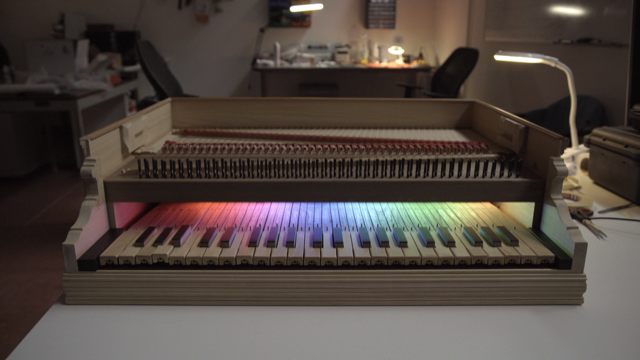
\includegraphics[width=1\linewidth]{img/mark2.png}
    \caption{Electronically Augmented Keyboard Interface. Colour LEDs are hidden from visitors by the name plate. These LEDs were used in the development and calibration process for visual feedback of key states.}
    \label{fig:mark2}
\end{figure}

With over fifty early keyboard instruments, primarily early plucked stringed keyboards of Italian origin, the Tagliavini Collection stands out as a valuable resource for musicologists, organologists and musicians alike. Preserving the instruments' authenticity was the cornerstone of Ferdinando Tagliavini’s vision. This guiding principle led him to collect instruments that could be restored to their playing condition after minimal intervention. 

In a collaboration between Museo San Colombano and the NEMUS project, we designed an electronically augmented replica of a historical harpsichord keyboard for interaction with digital musical instruments (Figure \ref{fig:mark2}). The goal was to enable visitors to experience the harpsichord’s unique vibro-tactile qualities without risking damage to the original artifacts and offer an immersive learning environment. The keyboard incorporates an optical sensor system and digital sound synthesis to replicate the physical feedback and acoustic response of an original 15th century harpsichord in the Italian style.

\begin{figure}
    \centering
    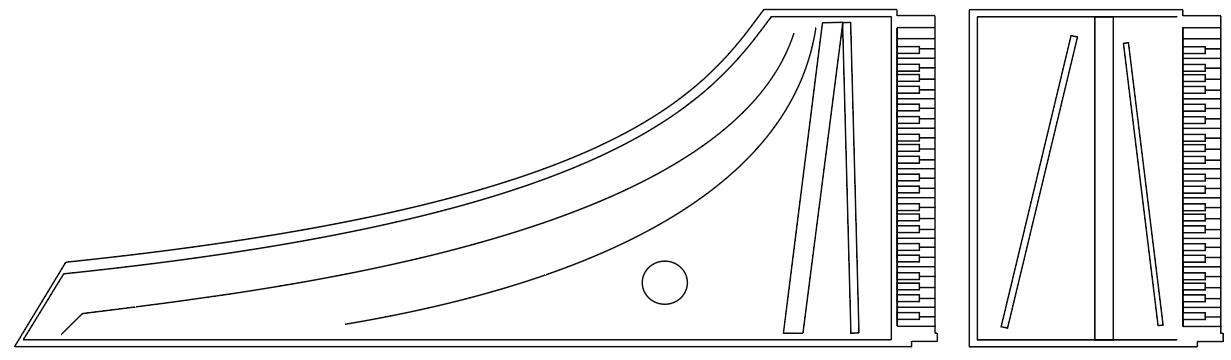
\includegraphics[width=1\linewidth]{img/comparison.png}
    \caption{Scale comparison between a 15th Century logarithmic shape and the new keyboard interface.}
    \label{fig:log-harp-comp}
\end{figure}

This new interface builds on the work of \textcite{mcalpine_sampling_2014} with the Benton Fletcher Collection. However, user tests identified a limitation: the commercially available weighted keys failed to provide an authentic sense of interacting with a historical plucked keyboard instrument \cite{mcalpine_sampling_2014}. The ``Tromba Moderna'' project \cite{baldwin_tromba_2016} approached the issue of musical heritage playability by recreating and augmenting a replica of a historical tromba marina. A piezo transducer was connected to a sound synthesis engine and a driver within the instrument to simulate the expected vibrations of a historical tromba marina. The new keyboard inherits some aspects from the Tromba Moderna project and addresses the limitations on the project by McAlpine. The optical sensing technique for the keyboard is adapted from a similar project on the piano by McPherson \cite{mcpherson_portable_2013}.

The aesthetics of the interface attempt to leverage the human tendency to be influenced by visual elements when making musical judgments \cite{tsay_sight_2013, fritz_player_2012,fritz_soloist_2014,fritz_listener_2017} and enhance its likelihood of being perceived as an `authentic' by visitors. The rectangular frame deviates from the traditional logarithmic (Figure \ref{fig:log-harp-comp}) form as the interface needed be compact enough not to compromise space for exhibition of the permanent display. The keyboard is hosted in the Oratory above the museum's main hall (Figure \ref{fig:installed}) alongside unique examples of the Italian Renaissance building tradition, including the 1547 harpsichord and the 1540 spinet by Alessandro Trasuntino.

\begin{figure}
    \centering
    \includegraphics[width=0.75\linewidth]{img/installation.png}
    \caption{Installation of the new keyboard in the Oratory, San Colombano.}
    \label{fig:installed}
\end{figure}

The interface is presently linked to a commercial software sampler; however, the ultimate aim is to make the sound of instruments in the collection that can no longer be maintained in playable condition accessible. Museum visitors are invited to play the interface and listen through a pair of headphones (Figure \ref{fig:user}).


\section{Conclusion}

The exhibition opened February 2025 and since then there have been two rounds of preliminary feedback collected. The first from a pool of 20 people -- consisting of staff, surveillance personnel and visitors who were given training on the system -- and expert feedback from curator Catalina Vicens and luthier Roberto Livi. The second round as part of a wider survey of the exhibition on a group of approximately 50 PhD students. This survey was in a five-point scale format the results of which are still being collected. From this group it was observed that some did not play the interface. When these visitors were later asked why they did not play the reasons given were that did not think they were allowed to touch the instrument. This could be considered in compliment for accuracy in the aesthetics of the keyboard but may also suggest a wider problem with  encouraging interaction in the museum context.

\begin{figure}
    \centering
    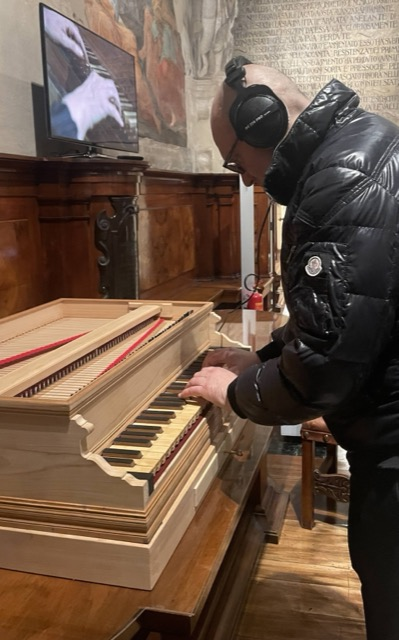
\includegraphics[width=0.33\linewidth]{img/exhibition-user-1.jpeg}
    \caption{Visitor to the exhibition demonstrating headphone setup.}
    \label{fig:user}
\end{figure}


Future design iterations will serve as a research probe to explore the unique characteristics of the harpsichord and its impact on performance much in the same manner as other musical haptics studies \cite{charalampos-saitis_musical_2018}. A longer discussion, but one going beyond the scope of this work, is whether the current setup or its future iterations may be effectively used to build legitimate replicas of historical musical instruments or even become a kind of new musical instrument altogether.

I argue here that a holistic conservation framework for musical instruments must integrate both values-based and living heritage perspectives. Such a synthesis acknowledges the physical realities of ageing instruments while honouring their performative and instructional roles. Moreover, this integration opens pathways to novel conservation strategies that extend beyond current paradigms.
